\documentclass[journal]{classes/IEEEtran}

\usepackage{cite}
\usepackage{amsmath,amssymb,amsfonts}
\usepackage{graphicx}
\usepackage{textcomp}
\usepackage{xcolor}
\usepackage{listings}

\lstset{
	basicstyle=\footnotesize\ttfamily,
	breaklines=true,
	frame=single,
	captionpos=b,
	tabsize=2,
	showstringspaces=false,
	commentstyle=\color{gray},
	keywordstyle=\color{blue},
	stringstyle=\color{red},
	frame=none
}

\begin{document}
	
	\title{Database Relationships in the Removals System}
	
	\author{Mindaugas Taujanskas}
	
	\maketitle
	
	\section{Introduction}

	\begin{figure*}[!t]
		\centerline{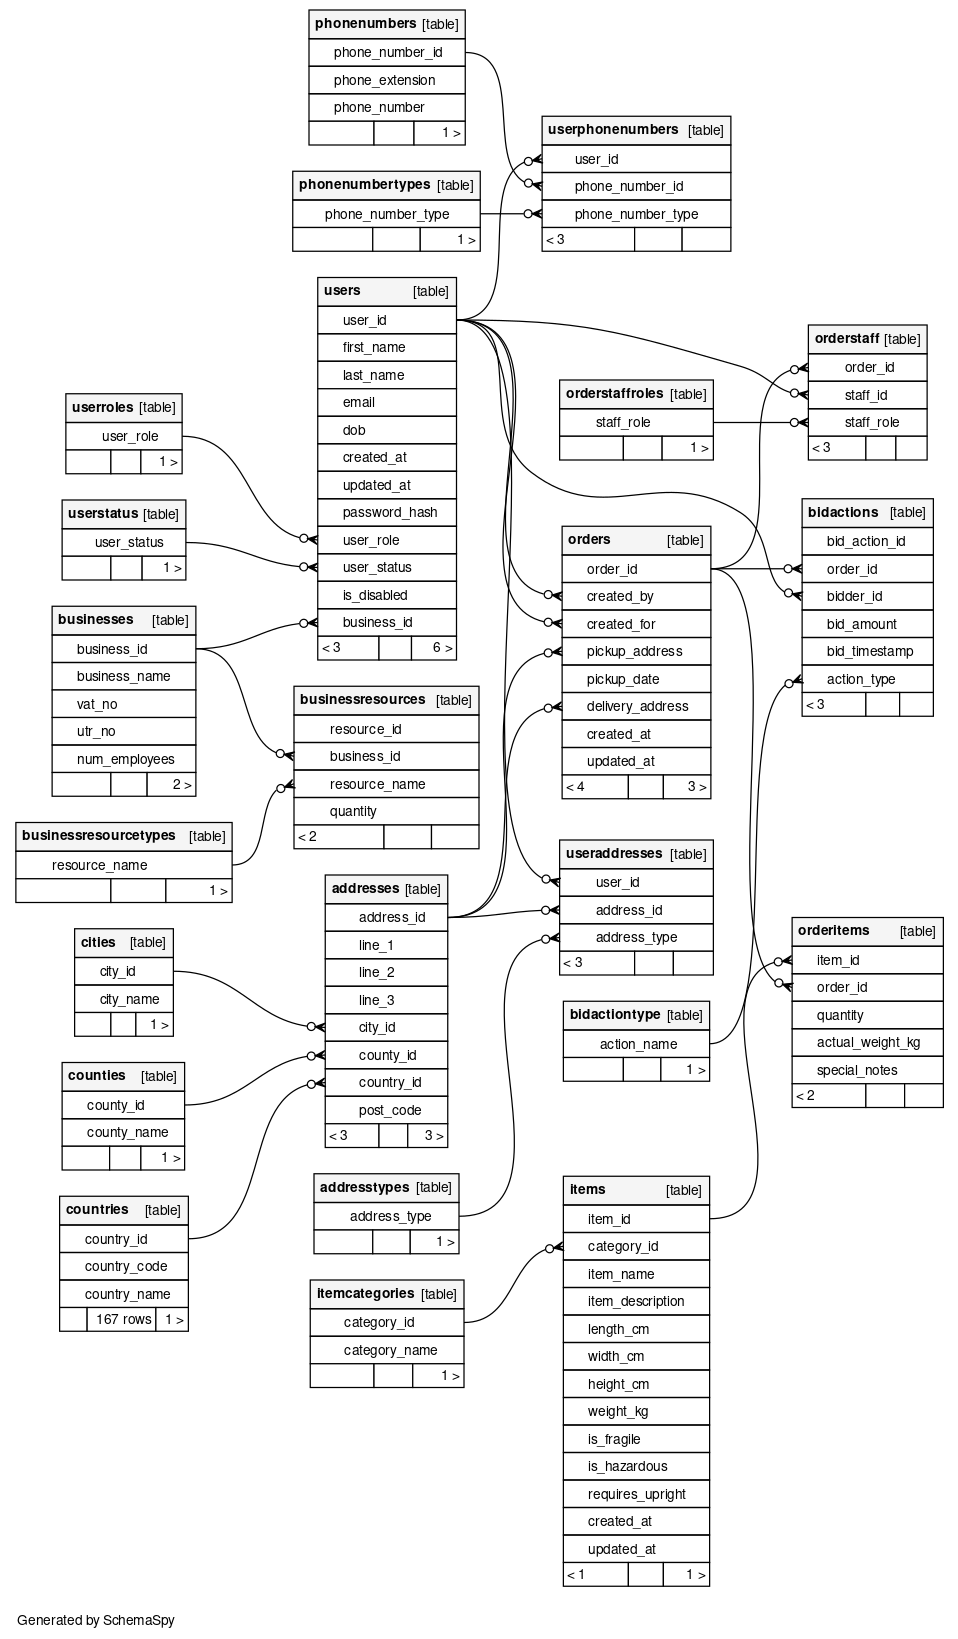
\includegraphics[width=\textwidth, height=\textheight]{resources/database.png}}
		\caption{Database diagram showcasing the interconnections between tables, and highlighting important constraints such as primary/foreign keys.}
		\label{fig:database}
	\end{figure*}
	
	Figure \ref{fig:database} demonstrates how the schema is constructed for the system. A majority of entity-attribute relationships (such as \texttt{Users} towards \texttt{UserAddresses}) are one-to-many to leave space for modularity down the road, e.g. allowing users to have multiple addresses.
	Simple one-to-one relationships are showcased in the \texttt{Addresses} table, which is defined as follows:
	
	\begin{lstlisting}[language=SQL]
CREATE TABLE Addresses (
	address_id INTEGER GENERATED ALWAYS AS IDENTITY,
	line_1 TEXT NOT NULL,
	line_2 TEXT,
	line_3 TEXT,
	city_id INTEGER NOT NULL,
	county_id INTEGER NOT NULL,
	country_id INTEGER NOT NULL,
	post_code CHAR(16) NOT NULL,
	
	CONSTRAINT PK_Addresses
	PRIMARY KEY (address_id),
	
	CONSTRAINT CHK_Addresses__line_length_1
		CHECK (LENGTH(line_1) <= 120),
	CONSTRAINT CHK_Addresses__line_length_2
		CHECK (COALESCE(LENGTH(line_2) <= 120, TRUE)),
	CONSTRAINT CHK_Addresses__line_length_3
		CHECK (COALESCE(LENGTH(line_3) <= 120, TRUE)),
	
	CONSTRAINT FK_Addresses_county
		FOREIGN KEY (county_id)
		REFERENCES Counties(county_id)
		ON DELETE RESTRICT,
	CONSTRAINT FK_Addresses_city
		FOREIGN KEY (city_id)
		REFERENCES Cities(city_id)
		ON DELETE RESTRICT,
	CONSTRAINT FK_Addresses_country
		FOREIGN KEY (country_id)
		REFERENCES Countries(country_id)
		ON DELETE RESTRICT
);
	\end{lstlisting}
	
	Each county, city, and country which is attributed to an address \textbf{must always exist}, as constrained by \lstinline[language=SQL]|ON DELETE RESTRICT|. Instead of a fixed-size declaration on the certain text fields, further length check-constraints exist to enable easier modification where necessary with the following migration:
	
	\begin{lstlisting}[language=SQL]
ALTER TABLE Addresses
DROP CONSTRAINT CHK_Addresses__line_length_1;

ALTER TABLE Addresses
ADD CONSTRAINT CHK_Addresses__line_length_1
CHECK (LENGTH(line_1) <= 60);
	\end{lstlisting}
	
	\section{How is data accessed?}
	
	Due to the nature of the architecture, confidential information would typically be easily accessible by a malicious user given that the database is locally-hosted. Preventative measures exist to minimise this risk through proper access management and setup. Once the database is created, the database administrator will run the following:
	
	\begin{lstlisting}[language=SQL]
FOR r IN
	SELECT tablename
	FROM pg_tables
	WHERE schemaname = 'public'
LOOP
	EXECUTE FORMAT('ALTER TABLE public.%I ENABLE ROW LEVEL SECURITY;', r.tablename);
END LOOP;

DROP ROLE IF EXISTS app_guest;

CREATE ROLE app_guest
LOGIN PASSWORD 'app_guest' NOINHERIT;

REVOKE ALL
ON ALL TABLES
IN SCHEMA public
FROM app_guest;

GRANT USAGE ON SCHEMA public TO app_guest;
GRANT EXECUTE
ON ALL FUNCTIONS
IN SCHEMA public
TO app_guest;
	\end{lstlisting}
	
	The \texttt{app\_guest} role acts as the controlled interface between the application and database, row-level security (RLS) is enabled to prevent users from viewing data to which they have no permission, as specified by their \texttt{Users.role} (customer or service-provider.)
	So, the principal mechanism by which data will be accessed in a controlled manner is via stored procedures which verify the user through session data. The first procedures called will be \texttt{login\_user} and \texttt{register\_user}, which return a JSON web token (JWT) and the user's corresponding role, so that the UI can display the correct view for each role.
	Subsequent attempts to call authenticated procedures which access restricted data must be supplemented with the aforementioned JWT, so that the database can validate access.
	
	\section{How is data validated?}
	Strict foreign key constraints and orphaning rules maintain database coherency by ensuring parent-child relationships are respected, check constraints on dimensional fields such as length/weight to ensure sane values, triggers on table insertions/updates validate that data remains coherent, e.g.:
	
	\begin{lstlisting}[language=SQL]
CREATE OR REPLACE FUNCTION user_update()
RETURNS trigger AS $$
BEGIN
	IF OLD.created_at IS DISTINCT FROM NEW.created_at THEN
		RAISE EXCEPTION
			'Cannot modify created_at timestamp';
	END IF;
	
	IF OLD.email IS DISTINCT FROM NEW.email
			AND NOT is_valid_email(NEW.EMAIL) THEN
		RAISE EXCEPTION
			'Newly updated email is invalid';
	END IF;
	
	NEW.updated_at = CURRENT_TIMESTAMP;
	RETURN NEW;
END;
$$ LANGUAGE plpgsql;

CREATE OR REPLACE FUNCTION user_before_insert()
RETURNS TRIGGER AS $$
DECLARE
	normalized_email TEXT;
BEGIN
	normalized_email := normalize_email(NEW.email);
	
	IF LENGTH(normalized_email) = 0 THEN
		RAISE EXCEPTION
			'Invalid email address: %', NEW.email;
	END IF;
	
	IF EXISTS (
		SELECT 1 FROM Users WHERE email = normalized_email
	) THEN
		RAISE EXCEPTION
			'Email address already exists: %', NEW.email;
	END IF;
	
	NEW.email := normalized_email;
	
	RETURN NEW;
END;
$$ LANGUAGE plpgsql;
	\end{lstlisting}
	
	When a \texttt{Users} entry is updated or inserted, a trigger will run to validate that the \texttt{created\_at} timestamp is not changed (as this field is immutable), and more importantly that the email remains valid. Although the email field is already designated as \lstinline[language=SQL]|UNIQUE|, there are various ways to write an email address which correspond to the same one--the \lstinline|normalize_email| procedure crudely transforms emails into their canonical form.
	
	A quintessential component which must remain coherent is an order's bid actions--ideally our architecture would have middle-ware to handle this crucial business logic, but even then some form validation would still occur at the database level. The code for this logic is fairly long and cryptic, but essentially the following constraints are validated:
	
	\begin{enumerate}
		\item Customer:
		\begin{enumerate}
			\item Must bid lower than the most recent price
			\item Cannot bid after accepting a price
			\item If accepting a bid, must accept a valid bid amount
		\end{enumerate}
		\item Service-provider:
		\begin{enumerate}
			\item Must bid higher than the most recent price
			\item Cannot accept bids on behalf of the customer
			\item Can withdraw valid bids they have created
		\end{enumerate}
	\end{enumerate}
	
	Crucially, bid history \textbf{must} be consistent and coherent to ensure regulatory compliance, there should be no procedure that allows the user to create a false image of the truth, or taint the bid history arbitrarily.
	
\end{document}